%----------------------------------------------------------------------------------------
%	PACKAGES AND THEMES
%----------------------------------------------------------------------------------------
\documentclass[aspectratio=169,xcolor=dvipsnames]{beamer}
\usetheme{Simple}

\usepackage{hyperref}
\usepackage{graphicx} % Allows including images
\graphicspath{ {./presentaciones/imgs/} }
\usepackage{booktabs} % Allows the use of \toprule, \midrule and \bottomrule in tables
\usepackage[spanish,mexico]{babel}

%----------------------------------------------------------------------------------------
%	TITLE PAGE
%----------------------------------------------------------------------------------------

% The title
\title[short title]{Analítica Visual para el Análisis de la Dinámica de la Calidad del Aire en la Zona Metropolitana del Valle de México}
\subtitle{}

\author[David Martínez] {J. David Martínez Cervantes}
\institute[CentroGeo] % Your institution may be shorthand to save space
{
    % Your institution for the title page
    Centro de Investigación en Ciencias de Información Geoespacial
    \vskip 3pt
}
\date{\today} % Date, can be changed to a custom date


%----------------------------------------------------------------------------------------
%	PRESENTATION SLIDES
%----------------------------------------------------------------------------------------

\begin{document}

\begin{frame}
    % Print the title page as the first slide
    \titlepage
\end{frame}

\begin{frame}{Marco Teórico}
    % Throughout your presentation, if you choose to use \section{} and \subsection{} commands, these will automatically be printed on this slide as an overview of your presentation
    \tableofcontents
\end{frame}

%------------------------------------------------
\section{Analítica Visual}
%------------------------------------------------

\begin{frame}{¿Qué es la Analítica Visual (AV)?}

Existen amplias definiciones que describen la AV: 

    \begin{block}{}
        Ciencia del razonamiento analítico, facilitado por interfaces visuales interactivas (Thomas and Cook, 2005)
    \end{block}
    
    \begin{block}{}
        Combina técnicas de análisis automatizado con visualizaciones interactivas para un efectivo entendimiento, razonamiento y toma de decisiones, basada en grandes y complejos conjuntos de datos (Keim et al., 2008)
    \end{block}

\end{frame}

%------------------------------------------------

\begin{frame}{Objetivos de la AV}

El objetivo de la AV se basa en la creación de técnicas y herramientas para permitir a la gente a:

    \begin{itemize}
        \item Sintetizar información y obtener una visión de datos que son masivos, dinámicos, ambíguos y muchas veces conflictivos.
        \item Detectar lo esperado y descubrir lo inesperado.
        \item Proveer evaluaciones oportunas, comprensibles y defendibles.
        \item Comunicar evaluaciones de forma efectiva para la acción.
    \end{itemize}
    
\end{frame}
%------------------------------------------------

\begin{frame}{Flujo de trabajo de la AV}

\begin{figure}[h]
\centering
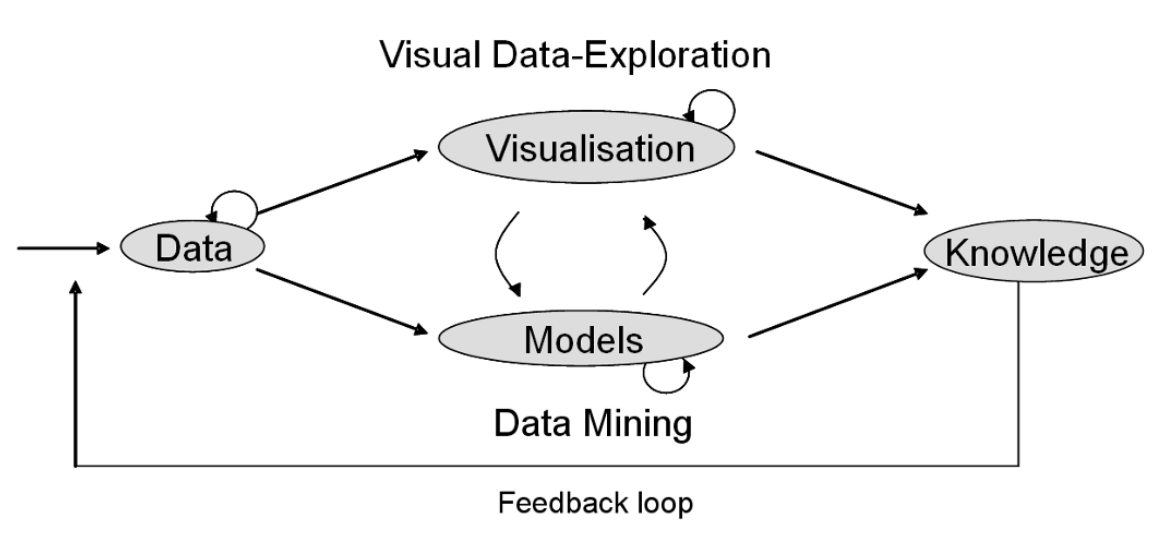
\includegraphics[scale=0.25]{feedback_loop_keim_2008.png}
\caption{Métodos de la integración visual y el análisis de datos automatizado (tomado de Keim et al., 2008).}
\end{figure}
    
\end{frame}
%------------------------------------------------

\begin{frame}{La AV como ciencia multidsciplinaria}

La AV es un campo interdisciplinario que incluye las siguientes áreas de enfoque:

    \begin{itemize} % The "c" option specifies centered vertical alignment while the "t" option is used for top vertical alignment
        \item Técnicas de razonamiento analítico.
        \item Representaciones visuales y técnicas interactivas.
        \item Representación y transformación de los datos.
        \item Producción, presentación y diseminación de los resultados.
    \end{itemize}
\end{frame}

%------------------------------------------------

\begin{frame}{AV y la integración con múltiples disciplinas}

\begin{figure}[h]
\centering
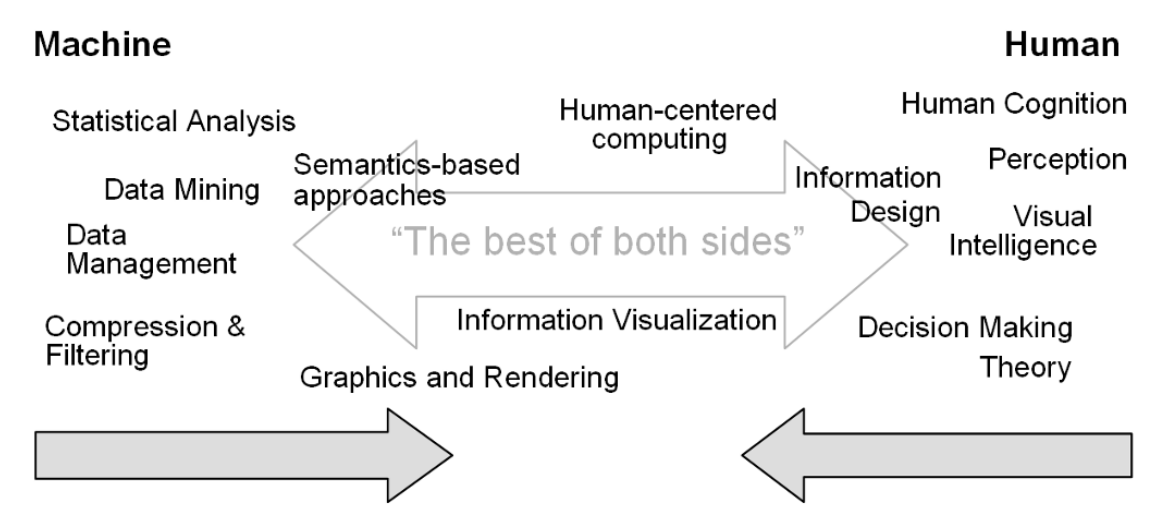
\includegraphics[scale=0.25]{va_integrates_human_machine_keim_2008.png}
\caption{La AV integra diversas disciplinas científicas para mejorar la división del trabajo entre el humano y la máquina (tomado de Keim et al., 2008).}
\end{figure}
    
\end{frame}
%------------------------------------------------
\section{Calidad del aire}
%------------------------------------------------

\begin{frame}{Referencias}
    % Beamer does not support BibTeX so references must be inserted manually as below

    \begin{itemize}
        \item D. Keim, G. Andrienko, J. D. Fekete, C. Görg, J. Kohlhammer, and G. Melançon. Visual analytics: Denition, process, and challenges. volume 4950 LNCS, 2008. doi: $10.1007/978-3-540-70956-5-7$.
        \item J. J. Thomas and K. A. Cook. Illuminating the path: The research and development agenda for visual analytics. IEEE Computer Society, 2005. ISSN 1664302X.
    \end{itemize}

\end{frame}

%------------------------------------------------

\end{document}